\documentclass[11pt,a4paper]{article}
% Working mathematical draft for the Numerical Practicum, UZH.
% Compile from the repository root containing figures/.
\usepackage[T1]{fontenc}
\usepackage[utf8]{inputenc}
\usepackage[english]{babel}
\usepackage{lmodern}
\usepackage{amsmath,amssymb,mathtools}
\usepackage{graphicx,booktabs,geometry,microtype,xcolor}
\usepackage{algorithm,algpseudocode}
\usepackage{pdflscape,caption,needspace,placeins,float}
\usepackage{hyperref}
\geometry{left=25mm,right=25mm,top=23mm,bottom=24mm}
\hypersetup{colorlinks=true,linkcolor=blue!40!black,urlcolor=blue!50!black}
\setlength{\parindent}{0pt}
\setlength{\parskip}{4pt}
\setlength{\abovedisplayskip}{6pt}
\setlength{\belowdisplayskip}{6pt}
\setlength{\textfloatsep}{11pt plus 2pt minus 2pt}
\setlength{\intextsep}{8pt plus 2pt minus 2pt}
\renewcommand{\topfraction}{0.92}
\renewcommand{\textfraction}{0.05}
\graphicspath{{figures/}}
\newcommand{\R}{\mathbb R}
\newcommand{\Th}{\mathcal T_h}
\newcommand{\V}{H_0^1(0,1)}
\newcommand{\ip}[2]{\langle #1,#2\rangle}
\newcommand{\norm}[1]{\left\lVert #1\right\rVert}
\newcommand{\abs}[1]{\left\lvert #1\right\rvert}
\newcommand{\sect}[1]{\Needspace{7\baselineskip}\section{#1}}
\newcommand{\subsect}[1]{\Needspace{5\baselineskip}\subsection{#1}}
\DeclareMathOperator*{\argmin}{arg\,min}
\algrenewcommand{\algorithmicrequire}{\textbf{Input:}}
\algrenewcommand{\algorithmicensure}{\textbf{Output:}}
\title{\vspace{-1.5cm}\textbf{Beyond the Obstacle}\\[5pt]
\large Adaptive Finite Elements and Nested Primal--Dual Active Sets}
\author{Victor Sieber\\\small Bachelor's student in Mathematics\\\small Numerical Practicum, University of Zurich}
\date{Last edited: \today}
\begin{document}
\maketitle
\vspace{-0.35cm}
\phantomsection
\section*{Abstract}
\addcontentsline{toc}{section}{Abstract}
% Intentionally blank until the project is finalized.
\vspace{0.45cm}
\tableofcontents
\vspace{0.1cm}

\sect{The obstacle problem}\label{sec:problem}
We model a string on $(0,1)$, fixed at its endpoints, under a load $f$. Its displacement $u$ must remain above an obstacle $\psi$. Set
\[
 V=H_0^1(0,1),\qquad K=\{v\in V:v\geq\psi\text{ a.e. on }(0,1)\}.
\]
Here $H_0^1(0,1)$ consists of functions with a square-integrable weak derivative and zero endpoint values. We choose obstacles with $\psi(0),\psi(1)\leq0$, so that $K$ is nonempty. Moreover, $K$ is convex: for $v,w\in K$ and $t\in[0,1]$,
\[
 tv+(1-t)w\ \geq\ t\psi+(1-t)\psi=\psi.
\]
The elastic energy and external work give
\[
 J(v)=\frac12\int_0^1|v'(x)|^2\,dx-\ip{f}{v},
 \qquad u=\argmin_{v\in K}J(v).
\]
If $f$ is a function, $\ip{f}{v}=\int_0^1 fv\,dx$. In one dimension, we may also use point forces: $\ip{\delta_\xi}{v}=v(\xi)$ for $\xi\in(0,1)$.

\textbf{Deriving the variational inequality.} For any $v\in K$, convexity gives $u+t(v-u)\in K$ when $0\leq t\leq1$. Since $u$ minimizes $J$, the right derivative satisfies
\[
 0\leq\left.\frac{d}{dt}J(u+t(v-u))\right|_{t=0}
 =\int_0^1 u'(v-u)'\,dx-\ip{f}{v-u}.
\]
Consequently, the weak obstacle problem is to find $u\in K$ such that
\begin{equation}\label{eq:VI}
 \boxed{\int_0^1u'(v-u)'\,dx\geq\ip{f}{v-u}\qquad\text{for every }v\in K.}
\end{equation}
We write $a(w,v)=\int_0^1 w'v'\,dx$. The \emph{Poincar\'e inequality}
\[
 \|v\|_{L^2(0,1)}\leq\frac1\pi\|v'\|_{L^2(0,1)}\qquad(v\in H_0^1(0,1))
\]
shows that the derivative seminorm controls the full $H^1$ norm. Hence $J$ is strictly convex on $V$ and the minimizer is unique.

\textbf{Contact and reaction.} At a point where $u>\psi$, small upward and downward variations are allowed, so the weak inequality becomes equality locally: $-u''=f$. On contact ($u=\psi$), only upward variations remain admissible. Their effect can be represented by a nonnegative \emph{reaction} $\lambda=-u''-f$. Thus, whenever these quantities are functions, we obtain
\[
 \underbrace{-u''=f+\lambda}_{\text{equilibrium}},\qquad
 \underbrace{u-\psi\geq0}_{\text{no penetration}},\qquad
 \underbrace{\lambda\geq0}_{\text{reaction}},\qquad
 \underbrace{\lambda(u-\psi)=0}_{\text{complementarity}}.
\]
On the \emph{free region} $u>\psi$, the reaction vanishes; on the \emph{contact region} $u=\psi$, the obstacle may exert a positive reaction. For point forces, the equilibrium equation is understood in the sense of distributions.

\sect{Finite-element discretization}\label{sec:fem}
\subsect{Meshes and the P1 and P2 bases}
Divide $[0,1]$ into $M$ elements
\[
 0=x_0<x_1<\cdots<x_M=1,\qquad T_i=[x_i,x_{i+1}],\quad h_i=x_{i+1}-x_i.
\]
Let $V_h\subset V$ contain continuous functions that are polynomial on each element and vanish at the two endpoints.

\textbf{$P_1$: one hat function per interior vertex.}
For each interior node $x_i$, define the \emph{global} nodal basis function
\[
 \varphi_i(x)=
 \begin{cases}
 (x-x_{i-1})/h_{i-1},&x\in[x_{i-1},x_i],\\
 (x_{i+1}-x)/h_i,&x\in[x_i,x_{i+1}],\\
 0,&\text{otherwise}.
 \end{cases}
\]
Thus $\varphi_i(x_j)=\delta_{ij}$, and
\[
 u_h(x)=\sum_{i=1}^{M-1}U_i\varphi_i(x),\qquad U_i=u_h(x_i),\qquad N=M-1.
\]
On an element $T_i$, only the two neighbouring hats contribute. With $s=(x-x_i)/h_i$,
\[
 u_h|_{T_i}(x)=U_i(1-s)+U_{i+1}s.
\]

\textbf{$P_2$: adding one midpoint to each element.}
We use the reference interval $\widehat T=[-1,1]$ with nodes $-1,0,1$, mapped to $T_i$ by
\[
 x=\frac{x_i+x_{i+1}}2+\frac{h_i}2y,\qquad y\in[-1,1].
\]
Construct the quadratic nodal functions as \emph{Lagrange polynomials}: each is one at its own reference node and zero at the other two. For example,
\[
 \widehat\varphi_L(y)=\frac{(y-0)(y-1)}{(-1-0)(-1-1)}=\frac12y(y-1).
\]
Analogously,
\[
 \widehat\varphi_M(y)=1-y^2,\qquad
 \widehat\varphi_R(y)=\frac12y(y+1).
\]
The local quadratic is $u_h|_{T_i}=U_i\widehat\varphi_L+U_{m_i}\widehat\varphi_M+U_{i+1}\widehat\varphi_R$, where $m_i=(x_i+x_{i+1})/2$. There are $M-1$ interior vertices and $M$ midpoints, hence $N=2M-1$ interior degrees of freedom.

\textit{Non-aligned mesh example.} For $M=20$ equal elements, $\alpha=1/3$ lies strictly inside $[0.30,0.35]$, not at the $P_1$ vertices or the $P_2$ midpoint $0.325$. Thus a free boundary or derivative jump need not be represented by a node. We will use this feature in the benchmark problems of Section~\ref{sec:benchmarks}.

\subsect{Stiffness matrix and constrained quadratic minimization}
Writing $u_h=\sum_{j=1}^N U_j\varphi_j$ in the energy gives
\[
 J_h(U)=\frac12U^TAU-F^TU,\qquad
 A_{ij}=\int_0^1\varphi_i'\varphi_j'\,dx,\quad F_i=\ip{f}{\varphi_i}.
\]
For $P_1$, the derivative of a hat is $1/h_{i-1}$ on its left element and $-1/h_i$ on its right element. Therefore,
\[
 A_{ii}=\frac1{h_{i-1}}+\frac1{h_i},\qquad
 A_{i,i-1}=-\frac1{h_{i-1}},\qquad
 A_{i,i+1}=-\frac1{h_i},
\]
with all other entries zero. In particular, on a uniform mesh of width $h$,
\[
 A_{P_1}=\frac1h
 \begin{pmatrix}
 2&-1&0&\cdots&0\\
 -1&2&-1&\ddots&\vdots\\
 0&-1&\ddots&\ddots&0\\
 \vdots&\ddots&\ddots&2&-1\\
 0&\cdots&0&-1&2
 \end{pmatrix}.
\]
For $P_2$, the chain rule gives $d/dx=(2/h_i)d/dy$, while $dx=(h_i/2)dy$. Therefore,
\[
 (A^{P_2}_{T_i})_{rs}=\frac2{h_i}\int_{-1}^1\widehat\varphi_r'(y)\widehat\varphi_s'(y)\,dy,
 \qquad r,s\in\{L,M,R\}.
\]
As $\widehat\varphi_L'=y-\tfrac12$, the $(L,L)$ entry is $(2/h_i)\int_{-1}^1(y-\tfrac12)^2dy=7/(3h_i)$. The neighbouring left--midpoint entry is
\[
 (A_{T_i}^{P_2})_{LM}=\frac{2}{h_i}\int_{-1}^1
 (y-\tfrac12)(-2y)\,dy=-\frac8{3h_i}.
\]
Similarly, the remaining entries give
\[
 A^{P_2}_{T_i}=\frac1{3h_i}
 \begin{pmatrix}7&-8&1\\-8&16&-8\\1&-8&7\end{pmatrix}.
\]
\textbf{From local to global ($P_2$).} Each element has three unknown values,
ordered as \emph{left vertex, midpoint, right vertex}:
\[
 \underbrace{(x_i,m_i,x_{i+1})}_{\text{element }T_i}
 \quad\longleftrightarrow\quad
 \underbrace{(2i,\,2i+1,\,2i+2)}_{\text{global positions}}.
\]
Place its $3\times3$ matrix into these rows and columns of the global
matrix \(\widetilde A\). Where two elements meet, \emph{add} their contributions.
For example, the interior vertex $x_i$ belongs to $T_{i-1}$ and $T_i$, so
\[
 \widetilde A_{2i,2i}=\frac{7}{3h_{i-1}}+\frac{7}{3h_i}.
\]
Thus $\widetilde A\in\R^{(2M+1)\times(2M+1)}$. Since
$u_h(0)=u_h(1)=0$, remove its first and last rows and columns:
\[
 \boxed{A\in\R^{(2M-1)\times(2M-1)}}.
\]
The same ``add at shared nodes'' rule was used for the $P_1$ matrix above.

The same assembly principle applies to $P_1$. For either degree, $A$ is symmetric and
\[
 c^TAc=\int_0^1\left|\left(\sum_{j=1}^N c_j\varphi_j\right)'\right|^2dx>0
 \quad\text{whenever }c\neq0,
\]
since a function in $H_0^1(0,1)$ with zero derivative must be zero.
Thus $A$ is positive definite. Let $z_i$ denote the interior $P_1$ vertices or $P_2$ vertices/midpoints and set $Z_i=\psi(z_i)$. We solve
\begin{equation}\label{eq:discrete}
 \boxed{\min_{U\in\R^N,\ U\geq Z}\bigl(\tfrac12U^TAU-F^TU\bigr).}
\end{equation}
Here $U\geq Z$ is imposed at the degrees of freedom. For $P_1$ it implies $u_h\geq I_h\psi$; for $P_2$, nodal feasibility alone need not imply pointwise feasibility between the nodes.

\textbf{Discrete KKT conditions.} Differentiate the discrete energy:
\[
 \nabla J_h(U)=AU-F=: \Lambda.
\]
If $U_i>Z_i$, we can vary $U_i$ slightly in either direction, hence $\Lambda_i=0$. If $U_i=Z_i$, only a positive variation is admissible, hence $\Lambda_i\geq0$. Together,
\begin{equation}\label{eq:KKT}
 \boxed{\Lambda=AU-F,\qquad U-Z\geq0,\qquad
 \Lambda\geq0,\qquad\Lambda_i(U_i-Z_i)=0\ \ (i=1,\ldots,N).}
\end{equation}
The vector $\Lambda$ is the \emph{dual residual}; it is not yet the nodal values of a multiplier function. In the Dirac example $f=f_{\rm reg}-2\delta_{\alpha}-\delta_{\beta}$, and the load vector is assembled as
\[
 F_i=\int_0^1f_{\rm reg}\varphi_i\,dx-2\varphi_i(\alpha)-\varphi_i(\beta).
\]
Even when $\alpha,\beta$ are not nodes, the basis values at those points are well-defined.

\sect{The primal--dual active-set method}\label{sec:pdas}
At each degree of freedom, the KKT system \eqref{eq:KKT} says that either
$U_i=Z_i$ (\emph{active/contact}) or $\Lambda_i=0$ (\emph{free}).
For any $c>0$, the four KKT conditions are equivalent to
\[
 \boxed{\Lambda_i=\max\{0,\Lambda_i-c(U_i-Z_i)\}.}
\]
\emph{Why?} Put $g_i=U_i-Z_i$. If $g_i>0$, KKT gives $\Lambda_i=0$,
so the right-hand side is $\max(0,-cg_i)=0$. If $g_i=0$, KKT gives
$\Lambda_i\geq0$, so the right-hand side is $\Lambda_i$.
Conversely, the maximum identity implies $\Lambda_i\geq0$;
if $\Lambda_i>0$ then $g_i=0$, while if $\Lambda_i=0$ then $g_i\geq0$.
Thus the identity also implies KKT.

This motivates the test
$\Lambda_i-c(U_i-Z_i)>0$ for an active degree of freedom.
We use $c=1$.
\begin{algorithm}[H]
\caption{Primal--dual active-set (PDAS) method}\label{alg:pdas}
\begin{algorithmic}[1]
\Require $A,F,Z$, parameter $c>0$, initial contact set $\mathcal C^0$
\For{$k=0,1,2,\ldots$}
 \State $\mathcal F^k\gets\{1,\ldots,N\}\setminus\mathcal C^k$ \Comment{free indices}
 \State $U_{\mathcal C^k}\gets Z_{\mathcal C^k}$ \Comment{enforce contact}
 \State Solve $A_{\mathcal F^k\mathcal F^k}U_{\mathcal F^k}
       =F_{\mathcal F^k}-A_{\mathcal F^k\mathcal C^k}Z_{\mathcal C^k}$
 \State $\Lambda\gets AU-F$
 \State $\mathcal C^{k+1}\gets\{i:\Lambda_i-c(U_i-Z_i)>0\}$
 \If{$\mathcal C^{k+1}=\mathcal C^k$ \textbf{and} the KKT residual is within tolerance}
   \State \Return $(U,\Lambda)$
 \EndIf
\EndFor
\end{algorithmic}
\end{algorithm}
\textbf{Why is stabilization a stopping criterion?}
Suppose $\mathcal C^{k+1}=\mathcal C^k=\mathcal C$.
For $i\in\mathcal C$, the algorithm sets $U_i=Z_i$, and stability gives
$\Lambda_i-c(U_i-Z_i)>0$, hence $\Lambda_i>0$.
For $i\notin\mathcal C$, the solved free equations imply
$\Lambda_i=(AU-F)_i=0$. Stability gives
$\Lambda_i-c(U_i-Z_i)\leq0$, hence $U_i-Z_i\geq0$.
In both cases $U_i-Z_i\geq0$, $\Lambda_i\geq0$, and
$\Lambda_i(U_i-Z_i)=0$: this is precisely \eqref{eq:KKT}.
In floating-point arithmetic we also verify KKT numerically
(the smooth code uses a $10^{-10}$ tie tolerance and a $10^{-8}$ KKT tolerance).

\textbf{Implementation and independent check.}
A cold start solves $A\widetilde U=F$ and initially selects
$\mathcal C^0=\{i:\widetilde U_i\leq Z_i\}$.
In the Dirac tests we use a tridiagonal $P_1$ solver and $P_2$ midpoint
elimination; the smooth test uses sparse free-set solves.
As an independent check, we also minimized the same quadratic objective
with SciPy's \texttt{L-BFGS-B}, using lower bounds and gradient $AU-F$
(\href{https://docs.scipy.org/doc/scipy/reference/optimize.minimize-lbfgsb.html}{SciPy reference}); the measurements appear in Section~\ref{sec:experiments}.

\sect{Residual-based error indicator and adaptive refinement}\label{sec:indicator}
\subsect{From jumps to an error residual}
On a $P_1$ element $T_i$, the computed slope is constant. At an interior
node, its jump is
\[
 s_i=u_h'|_{T_i}=\frac{U_{i+1}-U_i}{h_i},\qquad
 J_i=s_i-s_{i-1}=u_h'(x_i^+)-u_h'(x_i^-).
\]
We set $J_0=J_M=0$ because there is no neighbouring element at the boundary.
Our first (jump-only) indicator was
\[
 \eta_{T_i,\mathrm{jump}}^2=\frac{h_i}{2}(J_i^2+J_{i+1}^2).
\]
It responds to large changes in slope but ignores the force and obstacle reaction.
We now motivate the additional volume term.

\textbf{Step 1: express the error through the weak equation.}
Let $e=u-u_h$. For this derivation assume a regular load and an exact
reaction function $\lambda$, so that
$a(u,v)=\langle f+\lambda,v\rangle$ for all $v\in V$.
By the definition of $a$,
\begin{align*}
 \|e'\|_{L^2(0,1)}^2
 &=a(e,e)=a(u,e)-a(u_h,e)\\
 &=\langle f+\lambda,e\rangle-\int_0^1u_h'e'\,dx.
\end{align*}
The exact $\lambda$ is unknown. We therefore use a computable reconstruction
$\lambda_h$ (Section~\ref{sec:multiplier}) and add/subtract it:
\[
 \|e'\|_{L^2}^2
 =\underbrace{\langle f+\lambda_h,e\rangle-a(u_h,e)}_{\mathcal R_h(e)}
 +\langle\lambda-\lambda_h,e\rangle.
\]
The last term is the reconstruction error; we do not claim it vanishes.
We use $\mathcal R_h$ to \emph{motivate} a computable refinement indicator.

\textbf{Step 2: integrate by parts elementwise.}
For any $v\in V$ and $T_i=[x_i,x_{i+1}]$,
\begin{align*}
 -\int_{T_i}u_h'v'\,dx
 &=\int_{T_i}u_h''v\,dx-[u_h'v]_{x_i}^{x_{i+1}}\\
 &=\int_{T_i}u_h''v\,dx
   -u_h'(x_{i+1}^-)v(x_{i+1})+u_h'(x_i^+)v(x_i).
\end{align*}
On summing over elements, the endpoint terms vanish because $v(0)=v(1)=0$.
At $x_i$, the adjacent boundary terms combine into
\[
 \bigl(u_h'(x_i^+)-u_h'(x_i^-)\bigr)v(x_i)=J_iv(x_i).
\]
Thus, writing $(\lambda_h,v)=\int_0^1\lambda_hv\,dx$ for the regular case,
\[
 \boxed{\mathcal R_h(v)=
 \sum_{T\in\Th}\int_T\underbrace{(f+u_h''+\lambda_h)}_{R_T}v\,dx
 +\sum_{i=1}^{M-1}J_iv(x_i).}
\]
For $P_1$, $u_h''|_T=0$; for $P_2$, it is constant on each element.
The jump and volume terms are now both visible.

\subsect{Reconstructing the discrete multiplier}\label{sec:multiplier}
The PDAS output $\Lambda=AU-F$ is a vector, whereas $R_T$ requires a
function $\lambda_h(x)$. Define the linear functional on $V_h$ by
\[
 \ell_h(v_h)=a(u_h,v_h)-\langle f,v_h\rangle.
\]
For a basis function, $\ell_h(\varphi_i)=(AU-F)_i=\Lambda_i$.
Now equip the finite-dimensional space $V_h$ with the $L^2$ inner product.
By the \emph{Riesz representation theorem}, there exists a unique
$\lambda_h\in V_h$ such that
\[
 (\lambda_h,v_h)_{L^2}=\ell_h(v_h)
 \qquad\text{for every }v_h\in V_h.
\]
This is where Riesz enters: it replaces the \emph{functional} $\ell_h$
by a \emph{function} $\lambda_h$ representing it in the $L^2$ inner product.
Write $\lambda_h=\sum_{j=1}^N\mu_j\varphi_j$ and test with $v_h=\varphi_i$:
\[
 \sum_{j=1}^N\left(\int_0^1\varphi_j\varphi_i\,dx\right)\mu_j=\Lambda_i.
\]
With mass matrix $\mathsf M_{ij}=\int_0^1\varphi_i\varphi_j\,dx$,
\begin{equation}\label{eq:riesz}
 \boxed{\mathsf M\boldsymbol\mu=\Lambda.}
\end{equation}
Importantly, the dual entries $\Lambda_i$ are \emph{not} point values
$\lambda_h(z_i)$; solving this mass-matrix system produces the coefficient
vector of the reconstructed function.

\subsect{From the residual to the implemented indicator}
\textbf{Step 3: why subtract an interpolant?}
The discrete equation and the reconstructed multiplier imply
\[
 \mathcal R_h(v_h)=\langle f,v_h\rangle+(\lambda_h,v_h)-a(u_h,v_h)=0
 \qquad\text{for all }v_h\in V_h
\]
(for a regular load, up to numerical quadrature). However, the error
$e=u-u_h$ is generally \emph{not} in $V_h$. Choose an averaging interpolant
$\mathcal I_he\in V_h$, so that
\[
 \mathcal R_h(e)=\underbrace{\mathcal R_h(\mathcal I_he)}_{=0}
                     +\mathcal R_h(e-\mathcal I_he)
                  =\mathcal R_h(e-\mathcal I_he).
\]
\emph{Idea:} subtract a local average of $e$; only its variation over each
small element remains. This interpolant is used for the mathematical estimate,
not by the Python algorithm.

\textbf{Step 4: where do the factors $h_T$ come from?}
For an interval $\omega$ of length $h_\omega$, write
$\bar e_\omega=h_\omega^{-1}\int_\omega e(y)\,dy$.
Using the fundamental theorem of calculus and Cauchy--Schwarz,
\[
 \begin{aligned}
 |e(x)-\bar e_\omega|
 &=\left|\frac1{h_\omega}\int_\omega(e(x)-e(y))\,dy\right|\\
 &\leq\frac1{h_\omega}\int_\omega
             \left|\int_y^x e'(t)\,dt\right|dy
 \leq h_\omega^{1/2}\|e'\|_{L^2(\omega)}.
 \end{aligned}
\]
Taking the $L^2$ norm in $x$ gives
\[
 \|e-\bar e_\omega\|_{L^2(\omega)}
 \leq h_\omega\|e'\|_{L^2(\omega)}.
\]
This is the one-dimensional \emph{Poincar\'e inequality with the mean removed}.
For a suitable patchwise averaging interpolant, analogous local estimates are
\[
 \begin{aligned}
 \|e-\mathcal I_he\|_{L^2(T)}
 &\lesssim h_T\|e'\|_{L^2(\omega_T)},\\
 |(e-\mathcal I_he)(x_i)|
 &\lesssim h_T^{1/2}\|e'\|_{L^2(\omega_T)},
 \end{aligned}
\]
where $\omega_T$ consists of $T$ and its neighbours (the constants depend on
the local mesh geometry).

Set $w=e-\mathcal I_he$. Apply Cauchy--Schwarz separately to the
\emph{volume} and \emph{jump} terms of $\mathcal R_h(w)$:
\[
 \begin{aligned}
 \left|\int_T R_Tw\,dx\right|
 &\leq\|R_T\|_{L^2(T)}\|w\|_{L^2(T)}
 \lesssim\underbrace{h_T\|R_T\|_{L^2(T)}}_{\text{volume factor}}
          \|e'\|_{L^2(\omega_T)},\\
 |J_iw(x_i)|
 &\lesssim\underbrace{h_T^{1/2}|J_i|}_{\text{jump factor}}
          \|e'\|_{L^2(\omega_T)}.
 \end{aligned}
\]
Square these two residual factors. Each interior jump belongs to two
neighbouring elements, so assign half to each. This motivates our
\emph{implemented} indicator:
\begin{equation}\label{eq:indicator}
 \boxed{\eta_T^2=h_T^2\|f_{\rm reg}+u_h''+\lambda_h\|_{L^2(T)}^2
 +\frac{h_T}{2}(J_{T,L}^2+J_{T,R}^2),\qquad
 \eta_h=\Bigl(\sum_{T\in\Th}\eta_T^2\Bigr)^{1/2}.}
\end{equation}
The volume integral uses four-point Gauss--Legendre quadrature.
\emph{Caveat:} the exact--reconstructed multiplier difference in Step 1 has
not been bounded here. In the Dirac benchmark the point loads enter FEM
assembly but are not added explicitly to the indicator. Hence this is a
motivated refinement indicator, \emph{not} a general reliability theorem.

\subsect{Solve--estimate--mark--refine}
With maximum marking parameter $\theta=0.5$, mark the elements satisfying
\[
 \eta_T\geq\theta\max_{S\in\Th}\eta_S,
\]
then bisect every marked interval at its midpoint. Repeat
\[
 \boxed{\text{solve}\ \longrightarrow\ \text{estimate}\ \longrightarrow\ \text{mark}\ \longrightarrow\ \text{refine}}
\]
until $\eta_h\leq\mathrm{tol}$. This is the maximum-marking rule used in all adaptive experiments.

\sect{Nested initialization of PDAS}\label{sec:nested}
After refinement, the previous mesh solution is already a useful approximation to the new one. Instead of recomputing a cold initial guess, we transfer the coarse primal and dual information to the fine mesh.

\textbf{Primal initialization.} Let $H$ denote the coarse mesh and $h$ the refined mesh. Evaluate the old FE function $u_H$ at the new fine-grid nodes:
\[
 U_h^0=I_hU_H.
\]
Here $I_h$ is the nodal interpolation operator; coarse vertex values are retained.

\textbf{Dual initialization.} The coarse dual vector $\Lambda_H=A_HU_H-F_H$ consists of \emph{functional coefficients}, so simply interpolating its entries as if they were function values is not appropriate. We instead use the same $L^2$-Riesz reconstruction as in \eqref{eq:riesz}:
\[
 \underbrace{\mathsf M_H\boldsymbol\mu_H=\Lambda_H}_{\text{represent the coarse dual as a function}}
 \quad\longrightarrow\quad
 \underbrace{\boldsymbol\mu_h^0=I_h\boldsymbol\mu_H}_{\text{interpolate function values}}
 \quad\longrightarrow\quad
 \underbrace{\Lambda_h^0=\mathsf M_h\boldsymbol\mu_h^0}_{\text{recover fine dual}}.
\]
Combining both initializations gives the main transfer formula
\begin{equation}\label{eq:transfer}
 \boxed{U_h^0=I_hU_H,\qquad\Lambda_h^0=\mathsf M_h I_h\mathsf M_H^{-1}\Lambda_H.}
\end{equation}
These initial guesses determine the fine contact set
\[
 \mathcal C_h^0=\{i:(\Lambda_h^0)_i-c((U_h^0)_i-(Z_h)_i)>0\}.
\]
The subsequent PDAS steps are identical to the cold method: only the \emph{initial contact set} changes.

\begin{algorithm}[H]
\caption{Adaptive FEM with $L^2$-nested PDAS initialization}\label{alg:nested}
\begin{algorithmic}[1]
\Require Initial mesh $\mathcal T_0$, estimator tolerance $\varepsilon$, $\theta=0.5$
\State Solve on $\mathcal T_0$ by cold PDAS (Algorithm~\ref{alg:pdas})
\For{adaptive levels $\ell=0,1,2,\ldots$}
 \State Compute $\lambda_h$ and the indicators $\eta_T$ from \eqref{eq:indicator}
 \If{$\eta_h\leq\varepsilon$} \State \Return current mesh and $u_h$ \EndIf
 \State Mark by the maximum rule; bisect the marked elements
 \State Assemble $A_h,F_h,Z_h,\mathsf M_h$ on the refined mesh
 \State Transfer $(U_H,\Lambda_H)$ by \eqref{eq:transfer} and form $\mathcal C_h^0$
 \State Run PDAS (Algorithm~\ref{alg:pdas}) from $\mathcal C_h^0$
\EndFor
\end{algorithmic}
\end{algorithm}
For a controlled comparison, cold PDAS also solves the problem on each \emph{identical} adaptive mesh. We check that both results agree, so initialization affects iterations and timing but not approximation accuracy.

\sect{Construction of the benchmark problems}\label{sec:benchmarks}
\subsect{Dirac forces and an exact piecewise-quadratic solution}\label{sec:dirac}
Choose the constant obstacle $\psi=-1$ and the force
\[
 f=-6-2\delta_{\alpha}-\delta_{\beta},\qquad\alpha=\tfrac13,\quad\beta=\tfrac23.
\]
Away from the point loads, the free-region equation $-u''=-6$ implies $u''=6$, so the solution is quadratic on each free interval. We seek a contact interval $[\alpha,\gamma]$ where $u=-1$, so $u'=0$ on contact.

\textbf{Left free region.} Write $u(x)=3x^2+ax+b$. The endpoint condition $u(0)=0$ gives $b=0$, and continuity at $\alpha$ gives $u(\alpha)=-1$, hence $a=-4$. Therefore $u(x)=3x^2-4x$ for $x\leq\alpha$. Its derivative changes from $-2$ to $0$ at $\alpha$, so $[u']_{\alpha}=2$, corresponding to the force $-2\delta_{\alpha}$.

\textbf{Right free region.} Leaving contact smoothly at $\gamma$ gives $u(x)=-1+3(x-\gamma)^2$ until $\beta$. A force $-\delta_\beta$ requires $[u']_{\beta}=1$. Write $d=\beta-\gamma$; at $\beta$ we have $u(\beta)=-1+3d^2$, $u'(\beta^-)=6d$, $u'(\beta^+)=6d+1$. Continuing quadratically to $x=1$ and imposing $u(1)=0$ yields
\[
 0=(-1+3d^2)+(6d+1)\frac13+3\left(\frac13\right)^2
 =3d^2+2d-\frac13.
\]
The positive root is $d=(\sqrt2-1)/3$, hence $\gamma=\beta-d=1-\sqrt2/3$.

Together these conditions determine the exact solution
\[
 u(x)=\begin{cases}
 3x^2-4x,&0\leq x\leq\alpha,\\
 -1,&\alpha<x\leq\gamma,\\
 -1+3(x-\gamma)^2,&\gamma<x\leq\beta,\\
 3x^2+(2\sqrt2-5)x+2-2\sqrt2,&\beta<x\leq1.
 \end{cases}
\]
The reaction is $\lambda=6\mathbf1_{(\alpha,\gamma)}$ (a.e.), since $u''=0$ on contact and $u''=6$ elsewhere. At the point forces,
\[
 [u']_{\alpha}=2,\qquad[u']_{\gamma}=0,\qquad[u']_{\beta}=1.
\]
Thus $-u''=f+\lambda$ in distributions. The solution is continuous and piecewise quadratic but its derivative has jumps: a particularly informative test for localized refinement, especially with $P_2$ elements.

\subsect{A smooth manufactured bell with an active obstacle}\label{sec:smooth}
For a second test, we want \emph{no Dirac forces}, a non-polynomial exact solution, nonconstant obstacle, and nonzero reaction. We construct the example backwards: choose the solution and contact region first, then build the obstacle, multiplier and load to satisfy the KKT conditions.

\textbf{1. Prescribe the solution.} Choose a negative bell with zero endpoint values,
\[
 u(x)=-\sin(\pi x)e^{-6(x-1/2)^2},\qquad u(0)=u(1)=0.
\]
\textbf{2. Construct the obstacle.} Prescribe contact on $[1/3,2/3]$ using
\[
 d(x)=\max\{0,1-3x,3x-2\},\qquad\psi(x)=u(x)-d(x)^6.
\]
Here $d(x)=0$ exactly on $[1/3,2/3]$ and $d(x)>0$ outside. Thus $u-\psi=d^6\geq0$, with the desired contact set. The factor $3$ makes $d(0)=d(1)=1$, so $\psi(0)=\psi(1)=-1$; the sixth power makes the transitions $C^5$.

\textbf{3. Prescribe the reaction.} We need $\lambda\geq0$ only where $u=\psi$. Set
\[
 \lambda(x)=\left[36\left(x-\tfrac13\right)\left(\tfrac23-x\right)\right]_+^6,
 \qquad[t]_+=\max\{0,t\}.
\]
The factor $36$ normalizes the peak to $\lambda(1/2)=1$. Its support lies inside the contact interval, hence $\lambda(u-\psi)=0$.

\textbf{4. Determine the forcing.} Impose equilibrium $-u''=f+\lambda$, giving $f=-u''-\lambda$. With $t=x-1/2$,
\[
 u''(x)=e^{-6t^2}\left[(12+\pi^2-144t^2)\sin(\pi x)+24\pi t\cos(\pi x)\right].
\]
This verifies the continuous KKT conditions by construction. The exact $u$ is $C^\infty$ and non-polynomial; $\psi$, $\lambda$ and $f$ are $C^5$. In contrast with the Dirac benchmark, a $P_2$ element cannot reproduce the smooth exact solution exactly.

\sect{Numerical experiments}\label{sec:experiments}
For both benchmarks, report the $H^1$-seminorm error and $L^2$ error,
\[
 E_{H^1}=\left(\sum_{T\in\Th}\int_T|u'-u_h'|^2dx\right)^{1/2},\qquad
 E_{L^2}=\left(\sum_{T\in\Th}\int_T|u-u_h|^2dx\right)^{1/2}.
\]
We evaluate errors with 12-point elementwise Gauss--Legendre quadrature, splitting elements at the exact transition points. The smooth load uses 10-point quadrature; the indicator uses four-point quadrature. Error evaluation does not affect the computed meshes.

\subsect{Initial solver check: SciPy L-BFGS-B versus PDAS}
Before the adaptive studies, we compared PDAS with the L-BFGS-B method implemented in SciPy on a $P_1$ example with $f=-1$, $\psi(x)=x(1-x)-\tfrac32\alpha^2$ and $\alpha=0.2$. Both solve the same constrained minimization problem \eqref{eq:discrete}. Times are medians of seven \emph{wall-clock} runs per mesh (\texttt{perf\_counter}), unlike the later process-CPU timings.
\begin{table}[!htbp]\centering\small
\begin{tabular}{@{}rrrrrr@{}}\toprule
Elements & DOFs & L-BFGS-B iter. & PDAS iter. & L-BFGS-B [ms] & PDAS [ms]\\\midrule
20 & 19 & 12 & 4 & 0.266 & 0.074\\
80 & 79 & 35 & 13 & 0.901 & 0.376\\
320 & 319 & 169 & 51 & 9.322 & 7.534\\\bottomrule
\end{tabular}
\caption{Selected measurements from \texttt{experiments/benchmark\_solvers.py}. At 320 elements the discrete solutions differ by $8.82\times10^{-8}$; this is an independent solver check, not a broad speed comparison.}\label{tab:scipy}
\end{table}

\subsect{Smooth benchmark: approximation accuracy}\label{sec:exp-smooth}
For the problem in Section~\ref{sec:smooth}, uniform $P_1$ converges
approximately as $N^{-1}$ in $H^1$ and $N^{-2}$ in $L^2$; uniform $P_2$
gives $N^{-2}$ and $N^{-3}$. The adaptive curves have similar slopes,
while the reconstructed multiplier agrees closely with the exact reaction.

\begin{figure}[H]
\centering
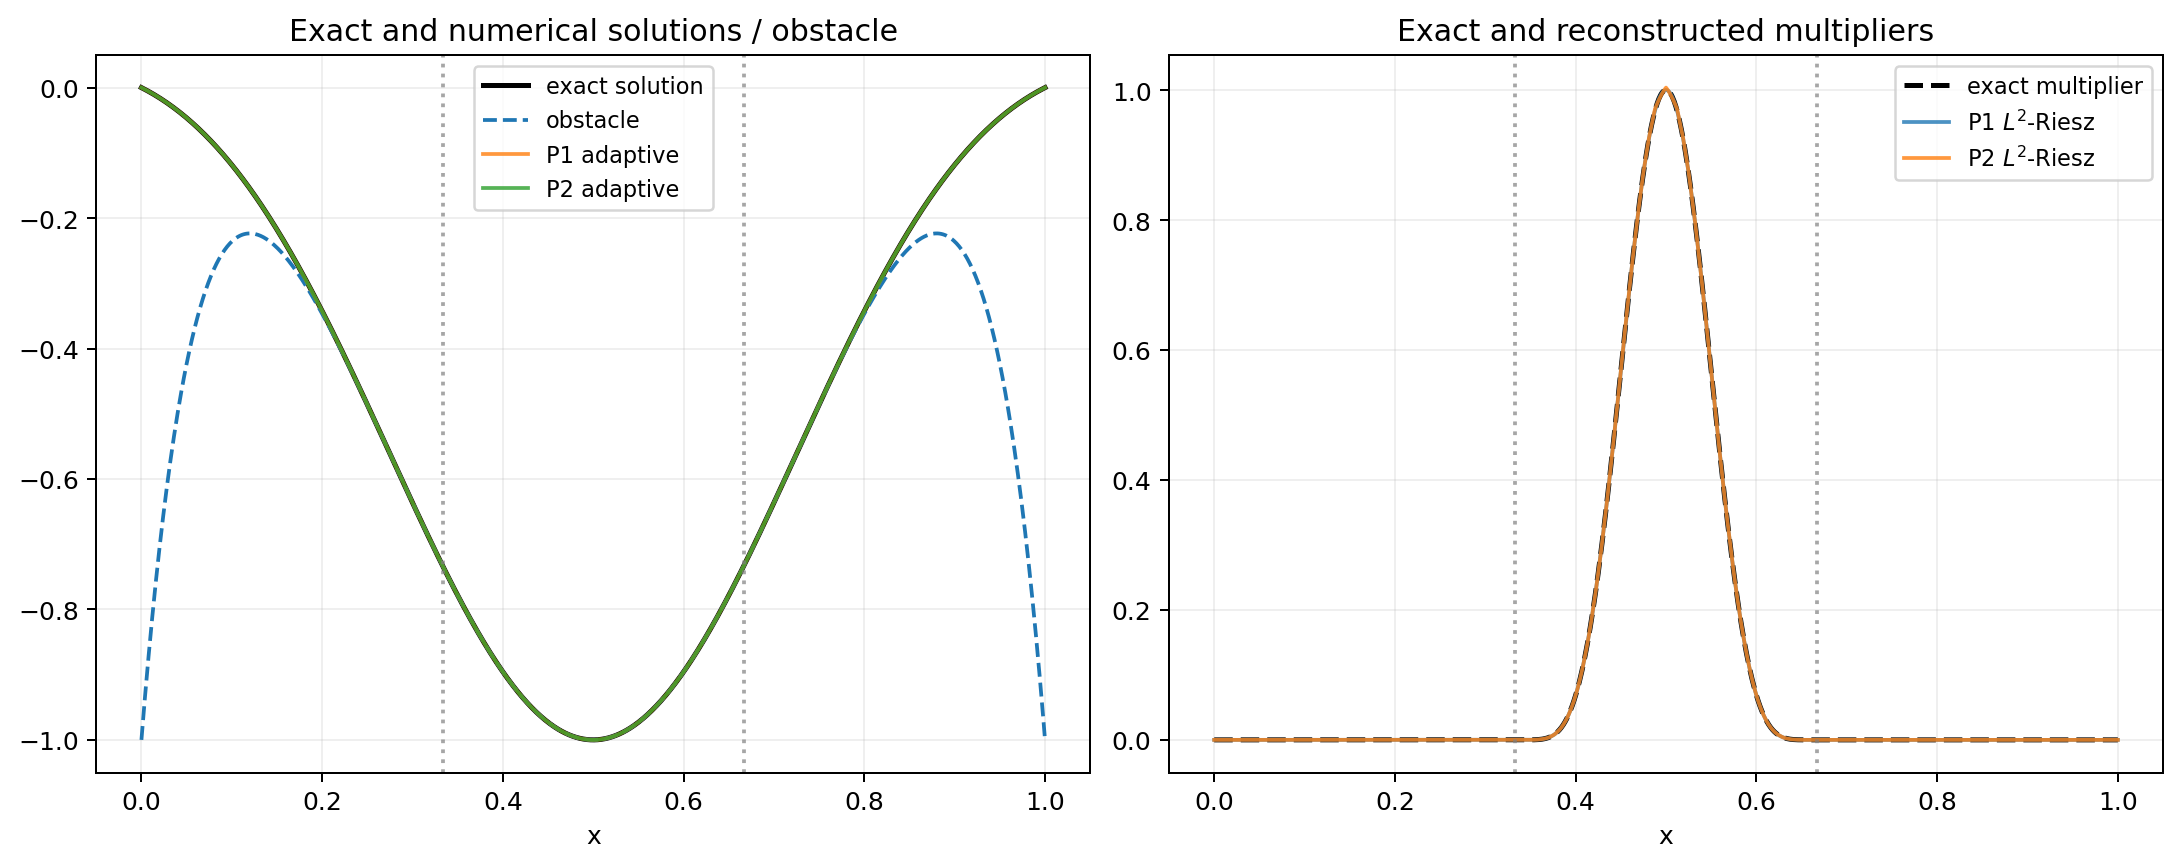
\includegraphics[width=0.89\linewidth]{smooth_bell_solution.png}
\caption{Smooth benchmark (Section~\ref{sec:smooth}): exact and FE solutions,
obstacle, and exact versus reconstructed multiplier.}\label{fig:smooth-solution}
\end{figure}
\vspace{-5pt}
\begin{figure}[H]
\centering
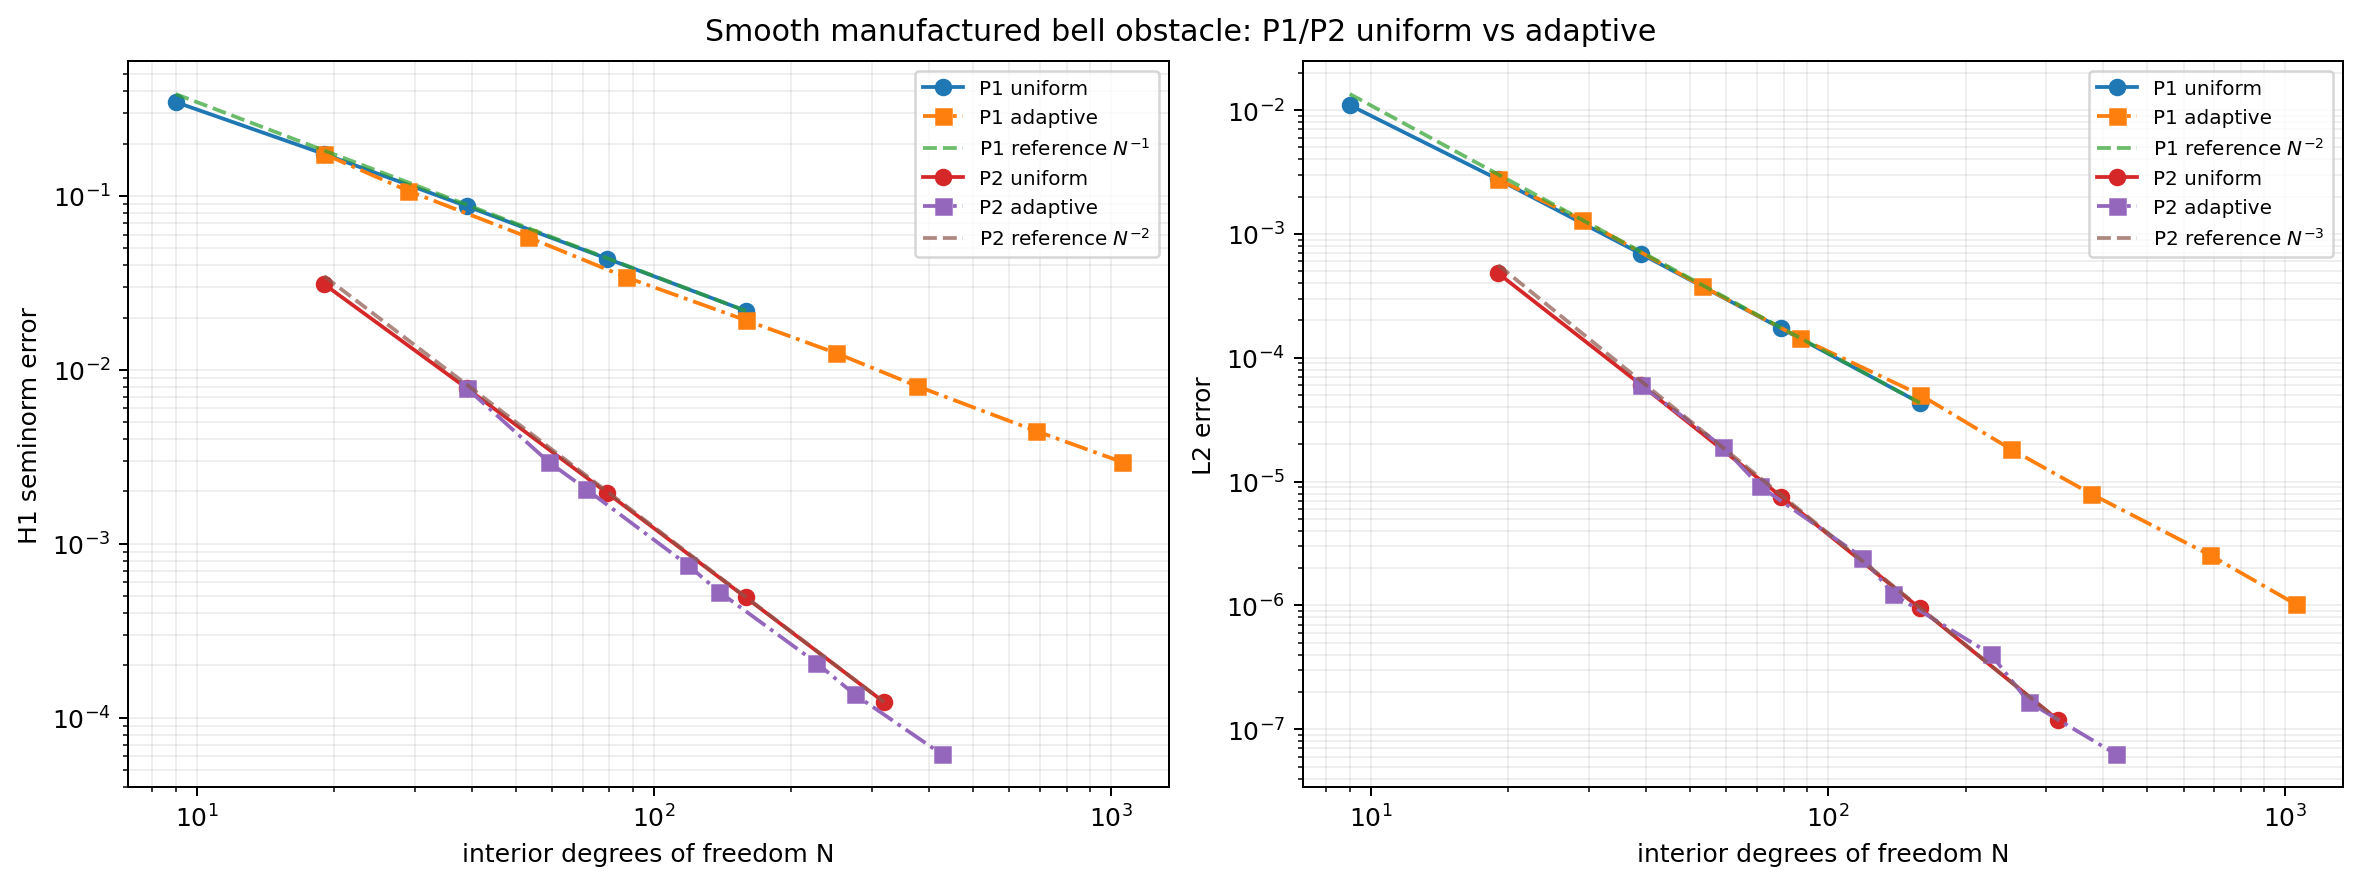
\includegraphics[width=0.89\linewidth]{smooth_bell_convergence.png}
\caption{Smooth $P_1/P_2$ errors versus DOFs: uniform and adaptive refinement
with reference slopes.}\label{fig:smooth-conv}
\end{figure}
\FloatBarrier

\subsect{Dirac benchmark: uniform versus adaptive refinement}\label{sec:exp-dirac}
For the singular problem in Section~\ref{sec:dirac}, uniform P1 and P2 produce observed rates near $N^{-1/2}$ in $H^1$ and $N^{-3/2}$ in $L^2$. Local refinement reduces the errors much faster for the piecewise-quadratic $P_2$ solution. These are benchmark-specific observations; unusually steep adaptive slopes are not claimed as general orders.
\begin{figure}[!htbp]\centering
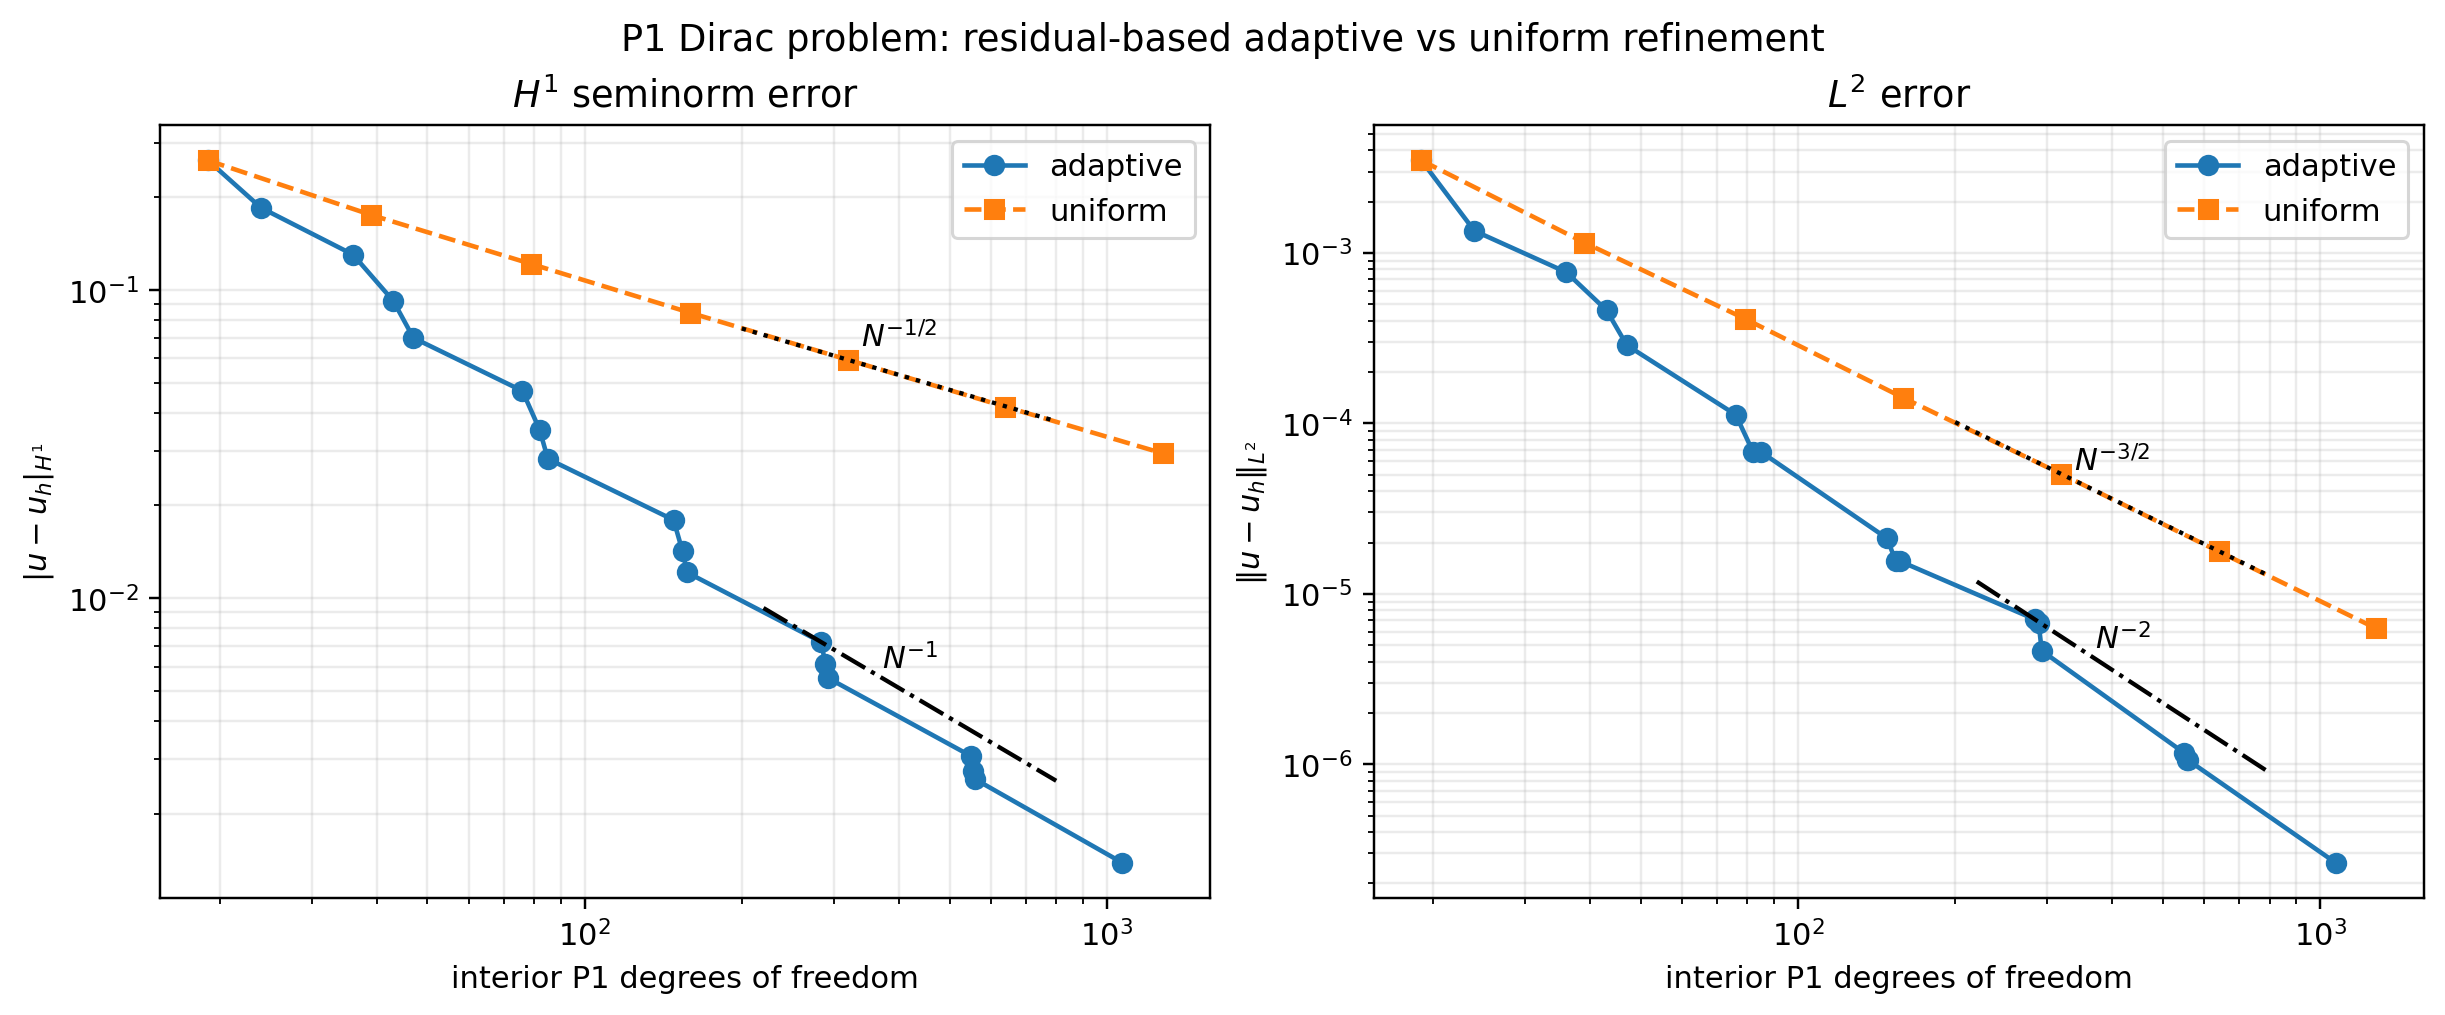
\includegraphics[width=0.87\linewidth]{p1_dirac_residual_adaptive_vs_uniform.png}
\caption{Dirac $P_1$: uniform and residual-adaptive errors, computed by elementwise Gaussian quadrature.}\label{fig:dirac-p1}
\end{figure}
\begin{figure}[!htbp]\centering
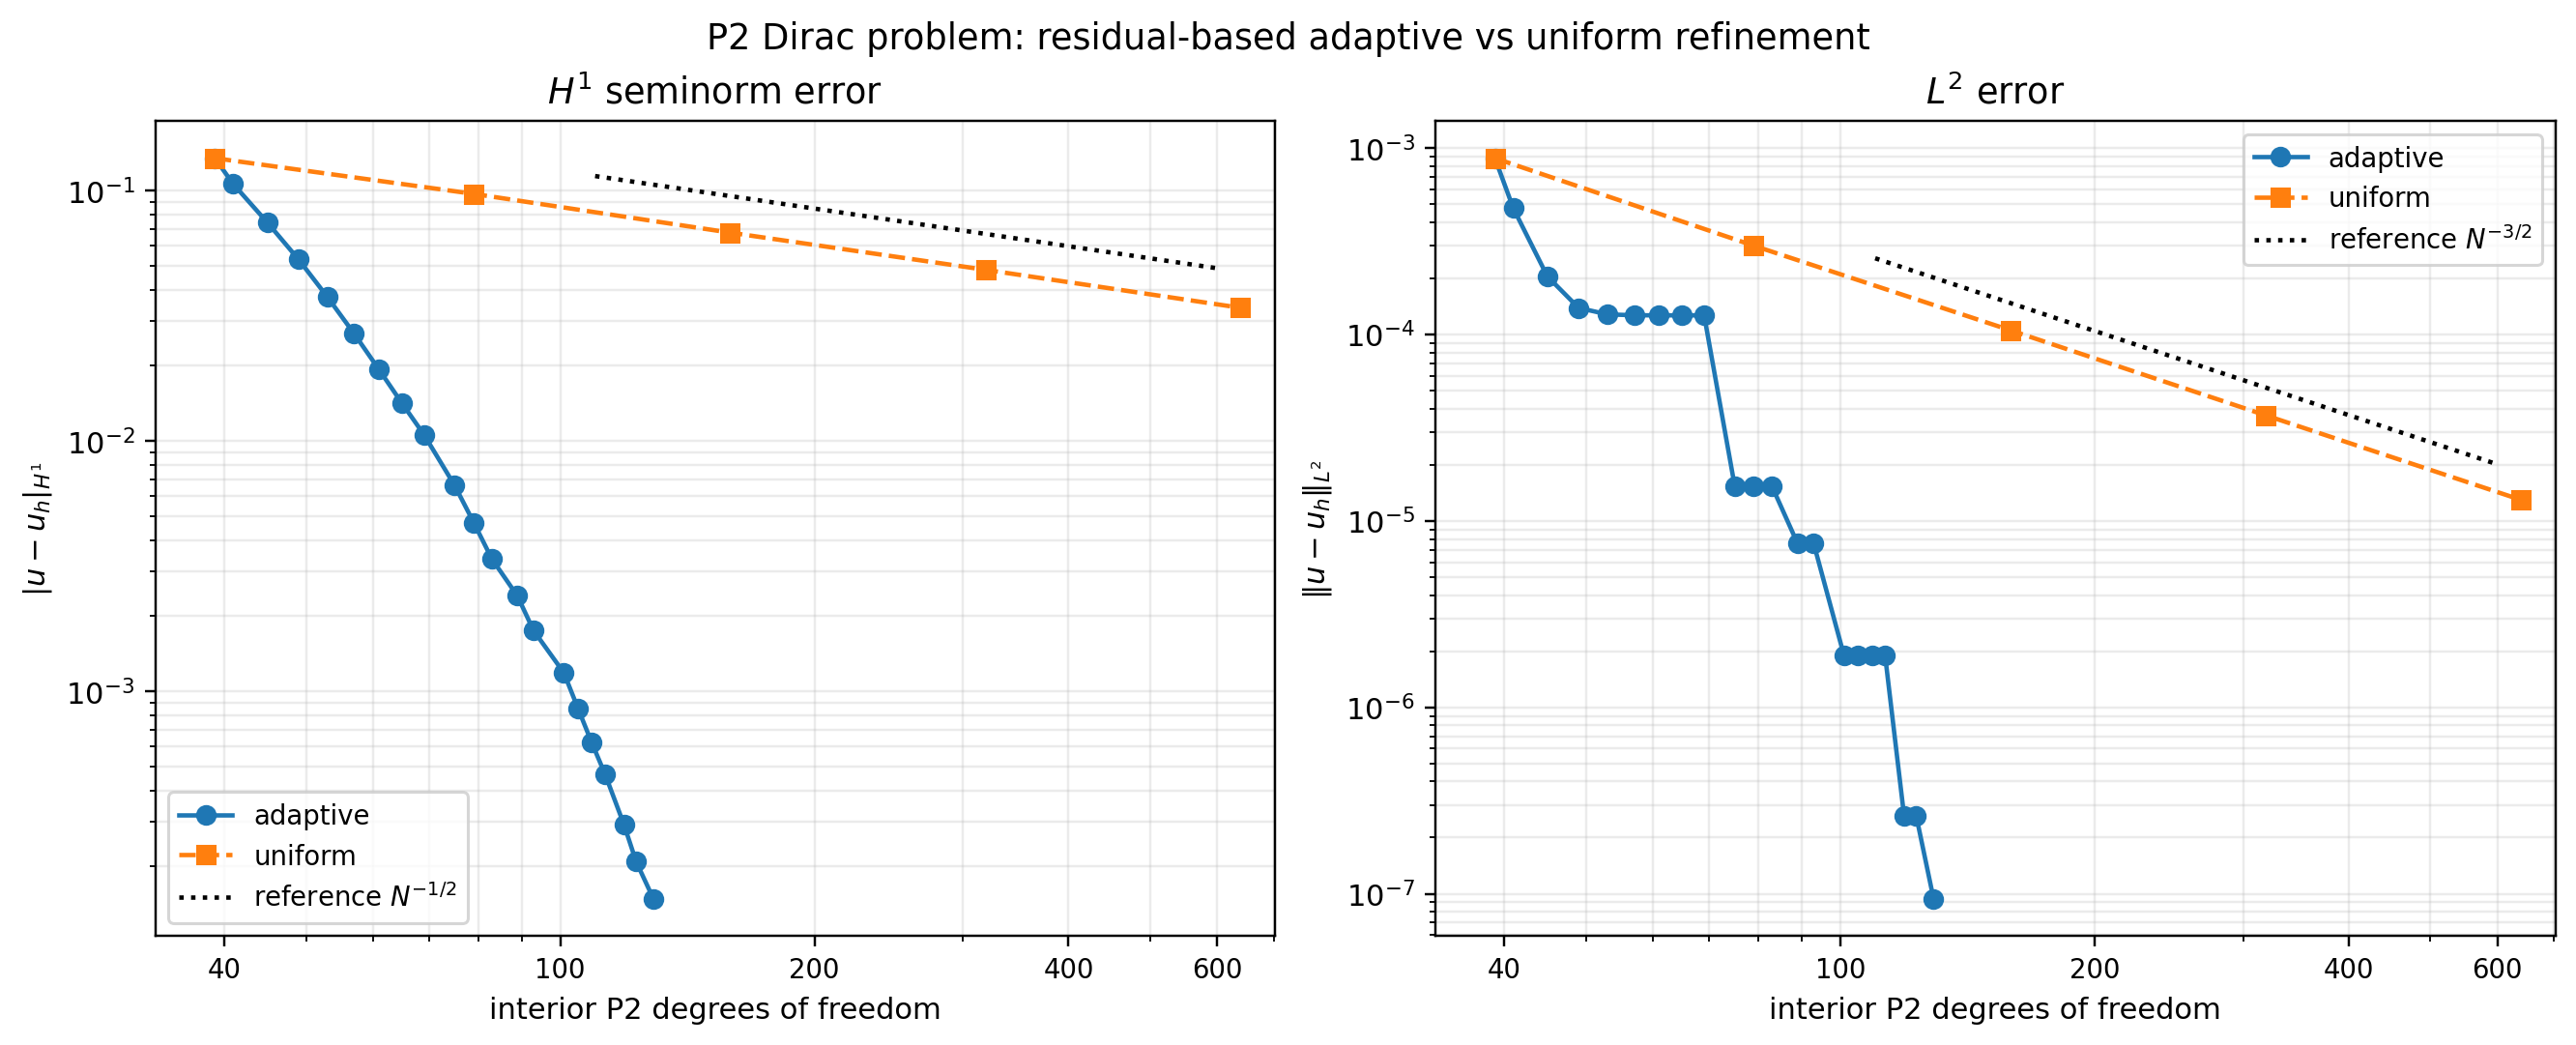
\includegraphics[width=0.87\linewidth]{p2_dirac_residual_adaptive_vs_uniform.png}
\caption{Dirac $P_2$: adaptive refinement concentrates DOFs near the derivative jumps and transition points.}\label{fig:dirac-p2}
\end{figure}
\FloatBarrier

\clearpage
\subsect{Efficiency of nested PDAS on identical adaptive meshes}\label{sec:exp-nested}
Now compare \emph{cold-start} and \emph{$L^2$-nested} PDAS on the same mesh at each adaptive level (a level is one mesh, before the next refinement). For each method and each level, the solver is timed five times with \texttt{process\_time()}; one plotted CPU point is the \emph{median of those five timings}, not a median across mesh levels. The coarse initial solve is charged to both methods.

For each benchmark, we also report the ratio
\[
 \text{solver-stage speedup}=
 \frac{\sum_{\ell=0}^L\operatorname{median}_{r=1,\ldots,5} t^{\mathrm{cold}}_{\ell,r}}
 {\sum_{\ell=0}^L\operatorname{median}_{r=1,\ldots,5} t^{\mathrm{nested}}_{\ell,r}}.
\]
Here $L+1$ is the number of mesh levels, $N$ is the number of interior FE degrees of freedom, and the ``final iterations'' refer to the \emph{last} adaptive mesh. Nested timings include primal/dual transfer and PDAS; neither method's timing includes assembly, the indicator, marking, refinement or error quadrature. The methods agree on the discrete solution (within $10^{-8}$), so accuracy curves are common to both.

\begin{table}[H]\centering\small
\begin{tabular}{@{}llrrrrrr@{}}\toprule
Case & FEM & Levels & Final $N$ & Final iter. cold/nested & Cold [s] & Nested [s] & Speedup\\\midrule
Smooth & $P_1$ & 9 & 1055 & $90/2$ & 0.05682 & 0.00688 & $8.3\times$\\
Smooth & $P_2$ & 8 & 427 & $86/15$ & 0.05336 & 0.01084 & $4.9\times$\\
Dirac & $P_1$ & 18 & 1071 & $245/5$ & 0.54651 & 0.01993 & $27.4\times$\\
Dirac & $P_2$ & 21 & 129 & $51/4$ & 0.05620 & 0.00644 & $8.7\times$\\\bottomrule
\end{tabular}
\caption{Sum of per-mesh median solver-stage CPU times (five repeats per method and mesh), with the final-mesh PDAS iteration counts.}\label{tab:nested}
\end{table}

In both test problems, nested initialization reduces the iteration count and measured solver cost.
These speedups compare the two initializations \emph{within} each benchmark and polynomial degree;
they are not end-to-end runtime gains or claims about different solver implementations.
Figures~\ref{fig:smooth-nested} and~\ref{fig:dirac-nested} show the full mesh histories.


\FloatBarrier
% Both six-panel efficiency comparisons are presented on equally oriented
% landscape pages, at the same scale, to keep every axis and legend legible.
\clearpage
\begin{landscape}
\thispagestyle{plain}
\begin{center}
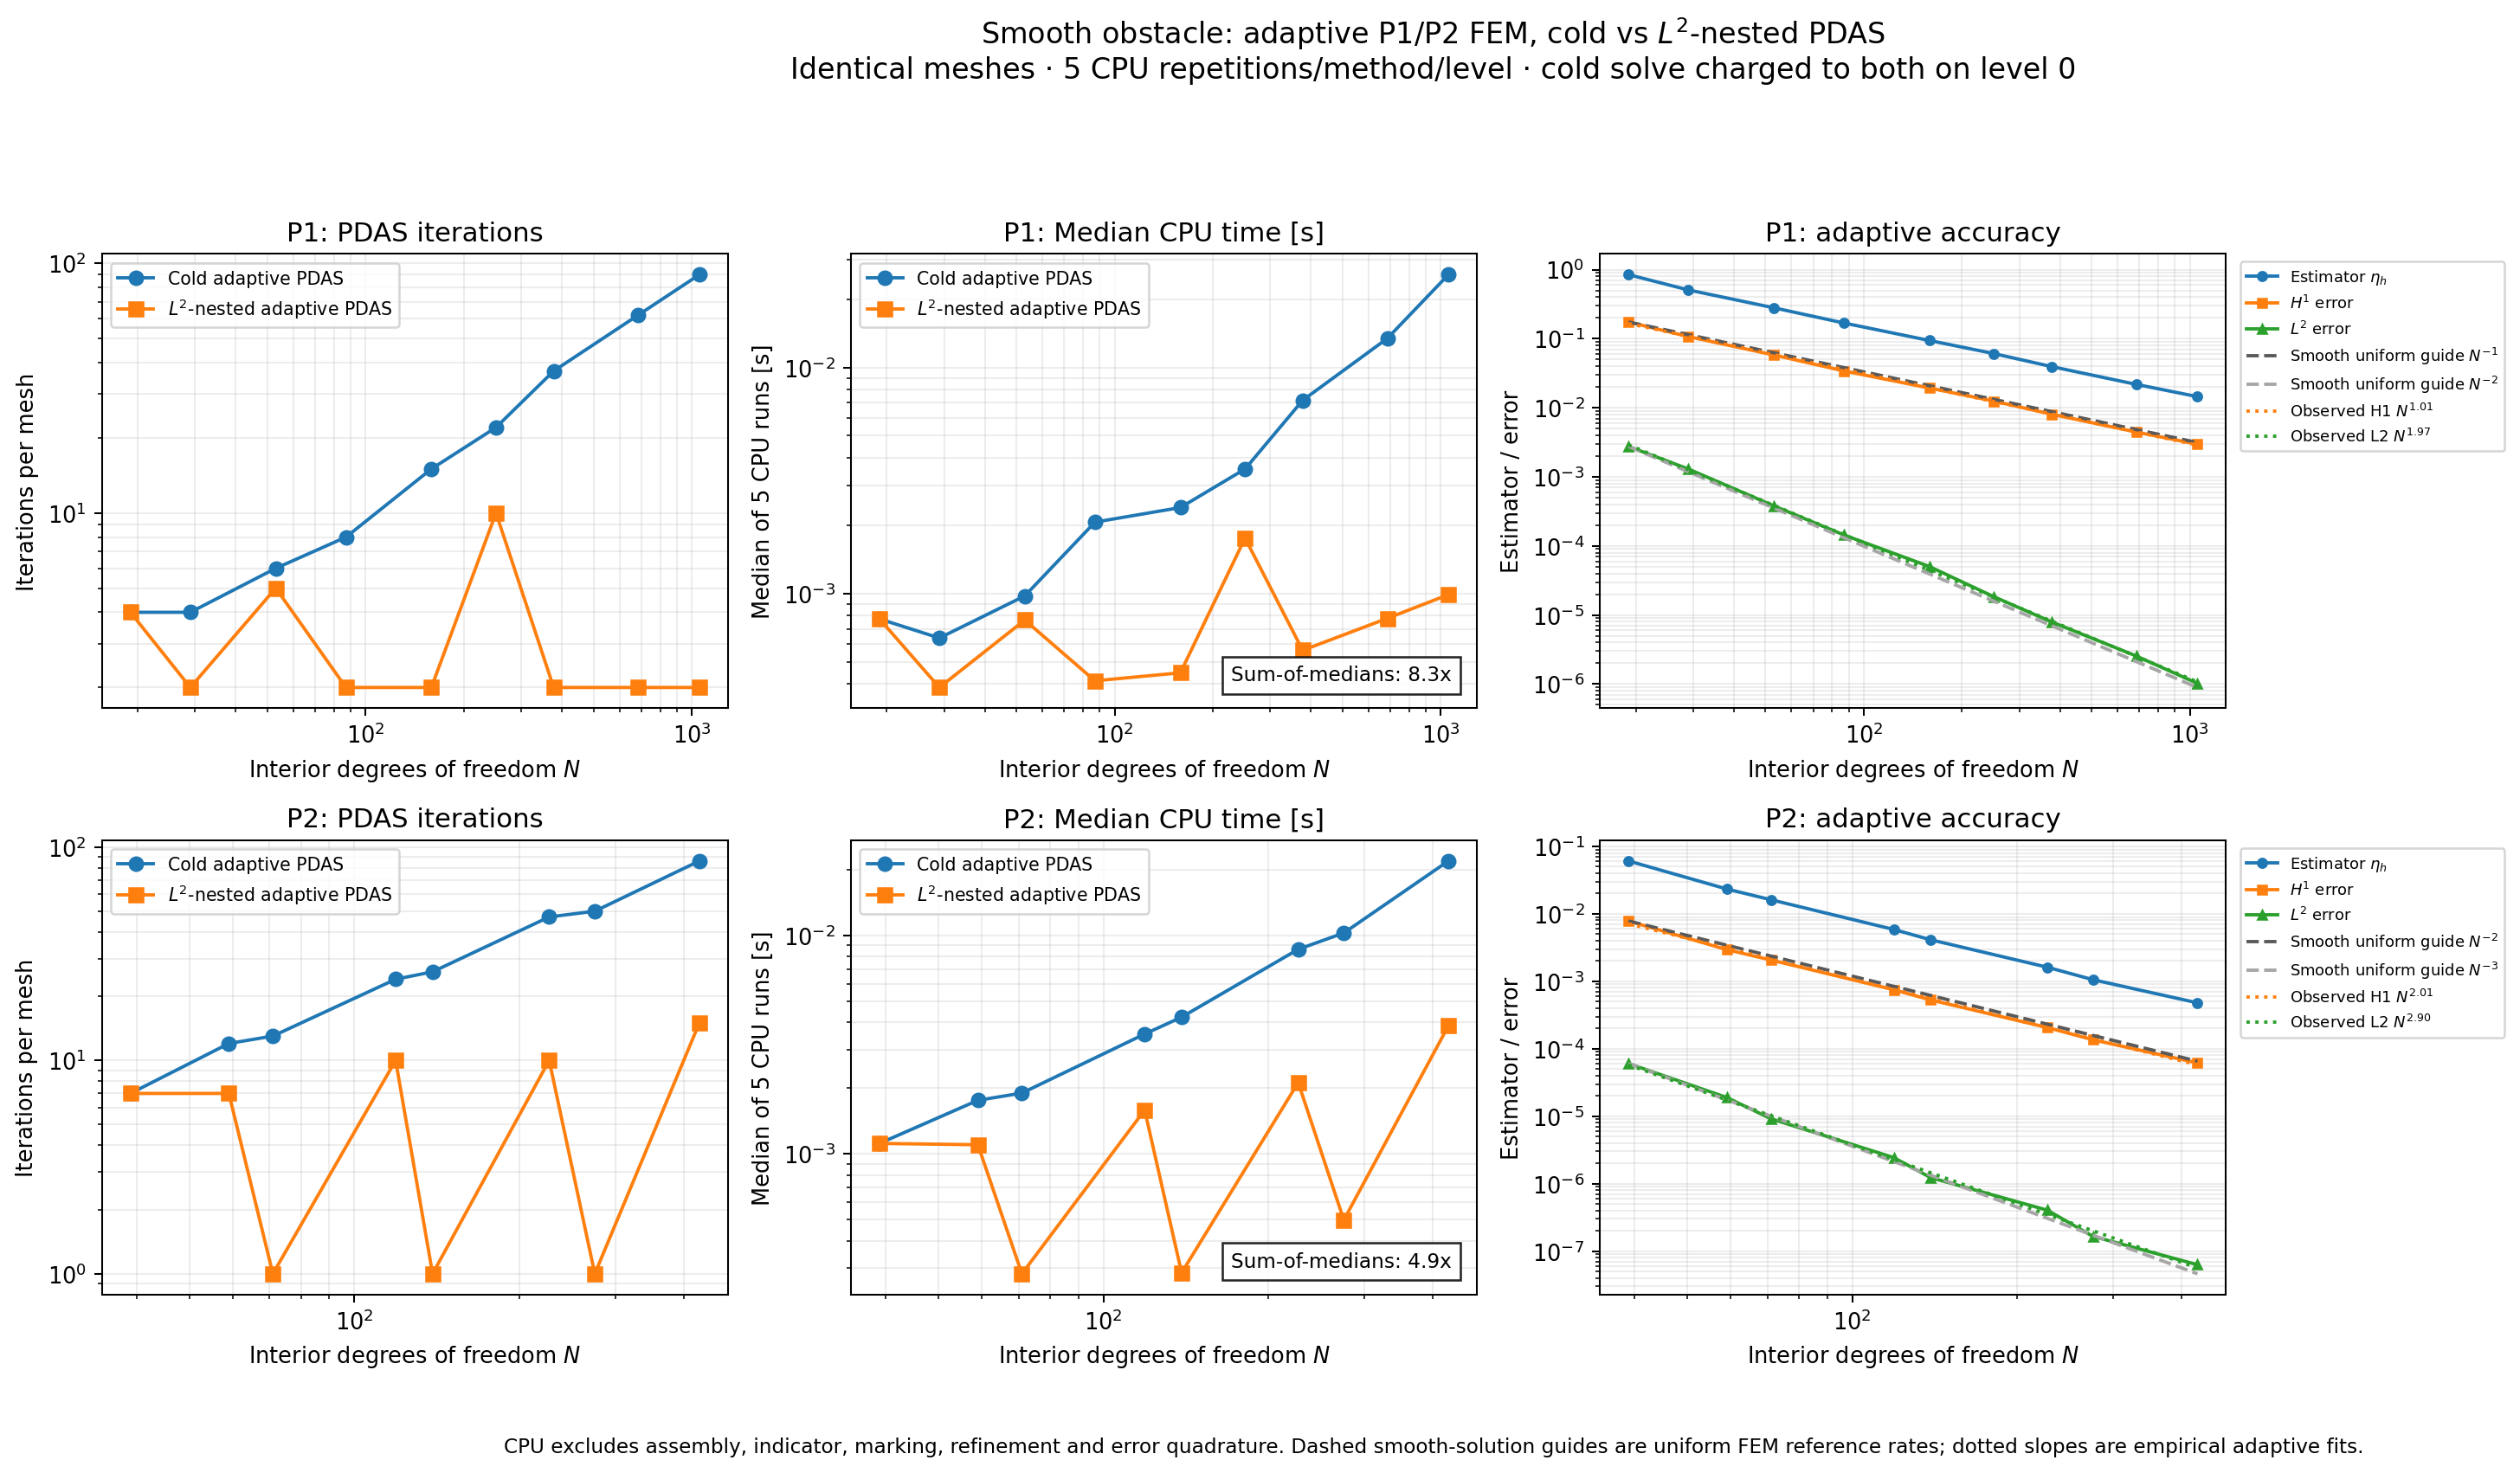
\includegraphics[width=0.98\linewidth,height=0.89\textheight,keepaspectratio]{smooth_nested_adaptive_p1_p2.png}
\captionof{figure}{Smooth benchmark (Section~\ref{sec:smooth}):
 cold versus $L^2$-nested PDAS on identical adaptive meshes for $P_1$ and $P_2$.}
\label{fig:smooth-nested}
\end{center}
\end{landscape}
\begin{landscape}
\thispagestyle{plain}
\begin{center}
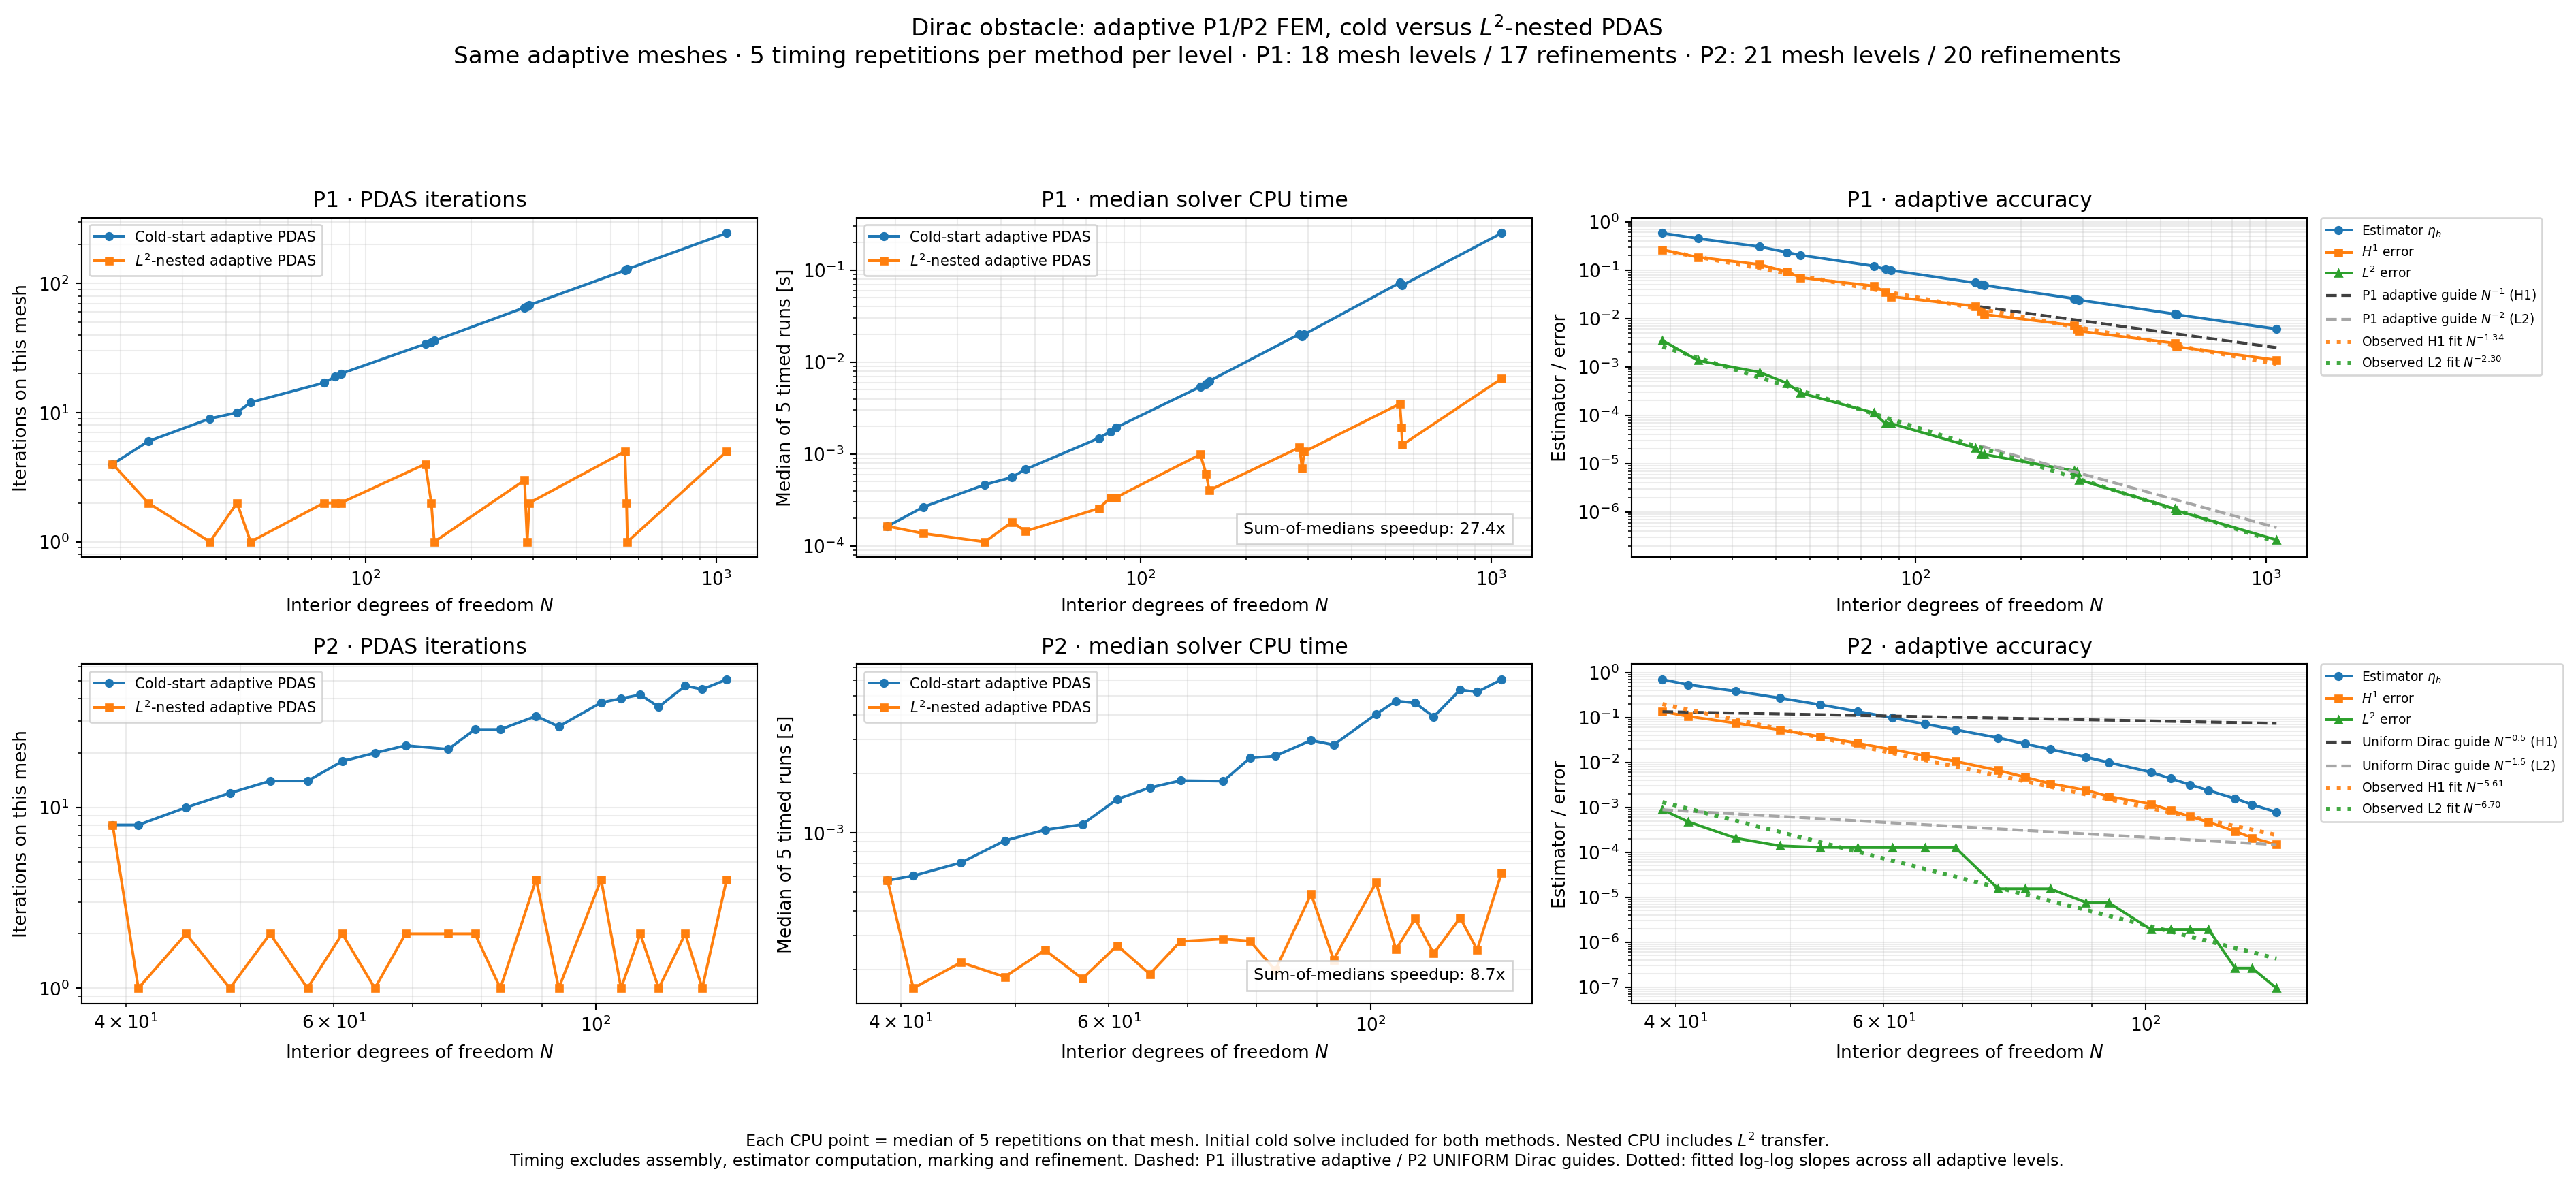
\includegraphics[width=0.98\linewidth,height=0.89\textheight,keepaspectratio]{dirac_nested_pdas_p1_p2_summary.png}
\captionof{figure}{Dirac benchmark (Section~\ref{sec:dirac}):
 cold versus $L^2$-nested PDAS on identical adaptive meshes for $P_1$ and $P_2$.
 Dashed reference guides and dotted finite-range fitted slopes have different meanings.}
\label{fig:dirac-nested}
\end{center}
\end{landscape}

\clearpage
\sect{Conclusion}
% Placeholder intentionally empty until the project is completed.
\subsect{Future work}
% Placeholder intentionally empty.
\subsect{Use of AI}
% Placeholder intentionally empty.
\subsect{Open questions}
% Placeholder intentionally empty.
\end{document}
